\documentclass[a4paper]{article}
\usepackage[english]{babel}
\usepackage[top=1.1cm,headsep=0cm,bottom=1.1cm,footskip=0cm,left=1cm,right=1cm]{geometry}
\usepackage{multicolrule} %다단 본문
\usepackage{fontspec}
\setmathtt{exprdgs-italic.ttf}[BoldFont = exprdgs-bolditalic.ttf]
\usepackage[colorlinks=true, allcolors=black]{hyperref}
\usepackage{wrapfig} %문단 내 이미지 삽입
\usepackage[abs]{overpic} %이미지 위 텍스트 삽입
\usepackage{graphicx,color} %색상
\usepackage[normalem]{ulem}%취소선
\usepackage{array} %표
\usepackage{mdframed, tcolorbox} %글상자
\usepackage{amsmath, amsfonts, amssymb, bm} %수식

\usepackage[yyyymmdd]{datetime}
\renewcommand{\dateseparator}{-}

\DeclareMathOperator{\arccsc}{arccsc}
\DeclareMathOperator{\arcsec}{arcsec}
\DeclareMathOperator{\arccot}{arccot}
\DeclareMathOperator{\csch}{csch}
\DeclareMathOperator{\sech}{sech}
\DeclareMathOperator{\arcsinh}{arcsinh}
\DeclareMathOperator{\arccosh}{arccosh}
\DeclareMathOperator{\arctanh}{arctanh}
\DeclareMathOperator{\arccsch}{arccsch}
\DeclareMathOperator{\arcsech}{arcsech}
\DeclareMathOperator{\arccoth}{arccoth}

\DeclareMathOperator{\snd}{s}
\DeclareMathOperator{\meter}{m}
\DeclareMathOperator{\cm}{cm}
\DeclareMathOperator{\mm}{mm}
\DeclareMathOperator{\mum}{\mu m}

\DeclareMathOperator{\newton}{N}
\DeclareMathOperator{\kn}{kN}
\DeclareMathOperator{\kgf}{kgf}

\DeclareMathOperator{\pa}{Pa}
\DeclareMathOperator{\kpa}{kPa}
\DeclareMathOperator{\mpa}{MPa}
\DeclareMathOperator{\gpa}{GPa}
\DeclareMathOperator{\mmhg}{mmHg}
\DeclareMathOperator{\knpm}{kN/m}

\DeclareMathOperator{\mps}{m/s}
\DeclareMathOperator{\mpss}{m/s^2}

\DeclareMathOperator{\dgr}{\!^\circ}
\DeclareMathOperator{\cel}{\!^\circ C}
\DeclareMathOperator{\fer}{\!^\circ F}
\DeclareMathOperator{\kel}{K}

\DeclareMathOperator{\kg}{kg}
\DeclareMathOperator{\kgpcm}{kg/m^3}
\DeclareMathOperator{\cmpkg}{m^3/kg}

\DeclareMathOperator{\nm}{N\cdot m}

\DeclareMathOperator{\watt}{W}
\DeclareMathOperator{\kw}{kW}
\DeclareMathOperator{\kwh}{kWh}

\DeclareMathOperator{\joule}{J}
\DeclareMathOperator{\kj}{kJ}
\DeclareMathOperator{\jpkg}{J/kg}
\DeclareMathOperator{\kjpkg}{kJ/kg}
\DeclareMathOperator{\kjpkk}{kJ/kg\cdot K}
\DeclareMathOperator{\kps}{kg/s}

\DeclareMathOperator{\satat}{sat\,@}
\DeclareMathOperator{\supat}{sup\,@}
\DeclareMathOperator{\comat}{com\,@}

\usepackage{polynom} %나눗셈 필산
\usepackage{cancel} %수식 약분선
\usepackage{titlesec} %섹션 이름 변경
\usepackage{kotex} %한글
\usepackage{fancyhdr} %페이지 넘버 편집
\pagestyle{fancy}
\renewcommand{\headrulewidth}{0pt}
\fancyhf{}
\fancyhead[R]{p.\thepage}
\fancyfoot[R]{\color{red}[\LaTeX]}

\setlength\columnsep{2cm}
\SetMCRule{
	width = 0.3mm,
	color-model = rgb,
	color = {0.9,0.9,0.9},
	line-style = dashed
}

\renewcommand{\section}[1] {
	\vspace{\baselineskip}
	\noindent\hspace{-1.0cm}\begin{overpic}{qframe.png}
		\put(8mm,-0.3mm){
			\begin{tcolorbox}[
				boxsep = 0mm,
				top = 0mm,
				bottom = 0mm,
				left = 0mm,
				right = 0mm,
				boxrule = 0mm,
				colback = white,
				colframe = blue,
				width = 2.2cm,
				height = 8mm,
				halign = center,
				valign = center,
				sharp corners = all,
				opacityfill = 0,
				fontupper = \bfseries
				]
				{[ #1 ]}
			\end{tcolorbox}
		}
	\end{overpic}
}

\makeatletter
\renewcommand{\maketitle}{\setlength{\parindent}{0pt}
	\begin{flushleft}
		\LARGE{\textbf{\@title}}\\
		\vspace{0.6cm}
		\LARGE{\qquad\@author}
		\vspace{0.5cm}
	\end{flushleft}
	\hspace{-1cm}\noindent\textcolor{red}{\rule{21cm}{0.5mm}}
}
\makeatother

\newcommand{\asw}[2]{
	\begin{flushright}
		{#1 \quad #2 \quad $\blacktriangleleft$}
	\end{flushright}
}

\newcommand{\solution}{\noindent\textbf{[풀이]}}

\title{열역학(이상훈 교수님)\hspace{5cm} 2025-1 중간고사 해설}
\author{기계공학부,\qquad 2022****,\qquad 2학년,\qquad ***\qquad\qquad{\normalsize 작성일 : \today}}
\date{}

\begin{document}

\maketitle

\begin{multicols*}{2}

\setlength{\parindent}{3mm}

\noindent* $\kappa_{\text{Air}} = 1.4$\quad * $R_{\text{Air}} = 0.2870\kjpkk$\\
*배점은 1$\sim$9번 1점, 10$\sim$16번 3점, 부분점수는 0.5점 단위

\section{Q1-3}
	아래 열역학 용어들을 영어로 쓰시오.\\[10pt]
	-공업 열역학 : engineering thermodynamics\\
	-임계점 : critical point\\
	-잠열 : latent heat

\section{Q4-8}
	아래 열역학 용어들의 정의를 쓰시오.\\[10pt]
	-내부에너지 : 시스템 내부의 미시적 에너지의 총합\\[10pt]
	-압축성 인자 : 실제기체가 이상기체로부터 벗어난 정도를 나타낸 인자\\[10pt]
	-밀폐계에서 에너지 보존 법칙 :
	$$\Delta E = Q - W$$
	특정한 시간동안 시스템의 에너지 변화량은 시스템이 같은 시간동안 받은 순 열과 같은 시간동안 시스템이 외부에 한 순 일의 차이와 같다.\\[10pt]
	-깁스의 상법칙 :
	$$f = c - p + n$$
	$f$ : 독립적 강성적 성질의 수\\
	$c$ : 시스템에 존재하는 성분의 수\\
	$p$ : 평형 상태에 있는 상의 수\\
	$n$ : 조성과 무관한 성질의 수
	
\section{Q9}
	$23\cel$를 화씨로 환산하라.
	\begin{align*}
		&32 + 23\times\frac{9}{5} = 73.4000 \approx 73.40\cel
	\end{align*}

\section{Q10}
	견고한 용기에 초기온도 $20\cel$, 초기압력 $180\kpa$의 이상기체 $12\kg$에 기체가 추가되어 $27\cel$,
	$250\kpa$로 변했을 때, 최종 기체의 질량을 구하시오.\\[10pt]
	\solution
	\begin{align*}
		&\mathtt{V} = \text{const.},\quad P_1 = 180\kpa,\quad P_2 = 250\kpa\\
		&m_1 = 12\kg\\
			&T_1 = (20 + 273.15)\kel = 293.15\kel\\
		&T_2 = (270+273.15)\kel = 300.15\kel\\
		&P\mathtt{V} = mRT,\quad \frac{\mathtt{V}}{R} = \frac{mT}{P} = \text{const.}\\
		&\frac{m_1T_1}{P_1} = \frac{m_2T_2}{P_2}
	\end{align*}
	\begin{align*}
		&m_2 = \frac{m_1T_1P_2}{T_2P_1} = \frac{(12)(293.15)(250)}{(300.15)(180)}\\
		&\quad = 16.27797213 \approx 16.278\kg
	\end{align*}
	\asw{}{$m_2 = 16.278\kg$}

\section{Q11}
	견고한 용기에 비체적이 $0.57015\cmpkg$, 압력이 $300\kpa$인 물 $1.5\kg$이 들어있다. 이때 ($a$) 물의 상태, ($b$) 내부 에너지를 구하시오. ($c$) 압력이 $500\kpa$로 상승했을 때 열전달량을 구하시오\\[10pt]
	\solution
	\begin{align*}
		&\mathtt{v} = 0.57015\meter^3,\quad P_1 = 300\kpa,\quad P_2 = 500\kpa\\
		&\mathtt{v}_f = \mathtt{v}_{f\,@\, 300\kpa} = 0.001073\cmpkg\\
		&\mathtt{v}_g = \mathtt{v}_{g\,@\, 300\kpa} = 0.60582\cmpkg\\
		&\mathtt{v}_f < \mathtt{v} < \mathtt{v}_g \quad\Rightarrow\quad \text{wet vapor}\\
		&x_1 = \frac{\mathtt{v} - \mathtt{v}_f}{\mathtt{v}_g - \mathtt{v}_f} = \frac{0.57015 - 0.001073}{0.60582 - 0.001073}\\
		&\quad = 0.9410166566 \approx 0.941
	\end{align*}
		\asw{($a$)}{습증기\;;\;$x=94.1\%$}
	\begin{align*}
		&u_{f1} = u_{f\,@\, 300\kpa} = 561.11\kjpkg\\
		&u_{fg1} = u_{fg\,@\, 300\kpa} = 1982.1\kjpkg\\
		&U_1 = mu_1 = m(u_{f1} + xu_{fg1})\\
		&\quad = (1.5)\{561.11 + (0.9410166566)(1982.1)\}\\
		&\quad = 3639.448673 \approx 3639.449\kjpkg
	\end{align*}
	\asw{($b$)}{$U = 3639.449\kj$}
	\begin{align*}
		&\left.\begin{array}{l}
			P_2=0.5\mpa\\
			\mathtt{v} = 0.57015\cmpkg
		\end{array}\right\}
		\;u_2 = 2883.0\kjpkg\\
		&Q = \Delta U = mu_2 - U_1 = (1.5)(2883.0) - 3639.449\\
		&\quad = 685.051000 \approx 685.051\kj
	\end{align*}
	\asw{($c$)}{$Q = 685.051\kj$}
	
\section{Q12}
	마찰이 없는 피스톤 실린더에 $0.5\mpa$, $350\cel$의 질소($\mathrm{N}_2$)가 들어있다. 일정한 압력을 유지하면서 $240\cel$로 냉각되었다. ($a$) 이때의 열전달량과 ($b$) 용기에 한 일을 구하시오. (비체적은 사용할 수 없음)
	\begin{align*}
		&R = 0.297\kjpkk\quad (\mathrm{N}_2) \\
		&c_p = 1.039\kjpkk\quad (\mathrm{N}_2)
	\end{align*}
	\solution
	\begin{align*}
		&q = c_p \Delta T = c_p(T_2 - T_1) = (1.039)(240-350)\\
		&\quad  = -114.29000 \approx -114.290\kjpkg\\
		&w = P\Delta\mathtt{v} = R(T_2 - T_1)= (0.297)(240 - 350)\\
		&\quad  = -32.67000 \approx -32.670\kjpkg
	\end{align*}
	\asw{}{$q = -114.290\kjpkg\,;\,w = -32.670\kjpkg$}
	
\section{Q13}
	마찰이 없는 피스톤 실린더에 $200\kpa$, $120\cel$의 이상기체가 $600\,\mathrm{L}$의 용기에 들어있다. 온도가 일정하게 유지되면서 체적이 $200\,\mathrm{L}$로 변해서 압축될 때, 용기에 한 일을 구하시오.\\[10pt]
	\solution
	\begin{align*}
		&P_1 = 200\kpa,\quad \mathtt{V}_1 = 0.6\meter^3,\quad \mathtt{V}_2 = 0.2\meter^3\\
		&mRT = P\mathtt{V} = \text{const.}\\
		&W = P_1\mathtt{V}_1\ln\frac{\mathtt{V}_2}{\mathtt{V}_1} = (200)(0.6)\ln\frac{0.2}{0.6}\\
		&\quad = -131.8334746 \approx -131.833\kj
	\end{align*}
	\asw{}{$W = -131.833\kj$}
	
\section{Q14}
	$300\,\mathrm{g}$의 물이 초기압력이 $500\kpa$, 초기온도 $145\cel$에서 $170\cel$로 일정한 압력을 유지하며 변한다. ($a$) 최초상태와 최종상태를 구하시오. ($b$) 열전달량을 구하시오. ($c$) 위 변화량을 $T$-$\mathtt{v}$ 선도에 나타내시오. (답을 구하는 과정에서 알아낸 모든 값들을 적당히 표현하시오.)\\[10pt]
	\solution
	\begin{align*}
		&T_{\satat 500\kpa} = 151.83\cel\\
		&T_{\satat 500\kpa} > T_1 = 145\cel\quad\Rightarrow\quad \text{압축액}\\
		&T_{\satat 500\kpa} < T_2 = 170\cel\quad\Rightarrow\quad \text{과열증기}
	\end{align*}
	\asw{($a$)}{압축액 $\to$ 과열증기}
	\begin{align*}
		&h_1 \approx h_{f @ 500\kpa} = 640.09\kjpkg
	\end{align*}
	@ $P=0.5\mpa$\quad\begin{tabular}{|c|c|}
		\hline
		$T\,[\,\cel]$\Large{\phantom{l}} & $h\,[\kjpkg]$\\
		\hline
		$151.83$ & $2748.1$\\
		$170.00$ & $h_2$\\
		$200.00$ & $2855.8$\\
		\hline
		\end{tabular}
	\begin{align*}
		&h_2 = \frac{170-200}{200-151.83}(2855.8-2748.1) + 2748.1\\
		&\quad = 2788.725057 \approx 2788.725\cmpkg\\
		&Q = \Delta H = m(h_2 - h_1) = (0.3)(2788.725 - 640.09)\\
		&\quad = 644.5905000 \approx 644.591\kj
	\end{align*}
	\asw{($b$)}{$Q = 644.591\kj$}
	($c$)\quad$\blacktriangleright$\vspace{-\baselineskip}
	\begin{center}
		\includegraphics{img/q14-0.png}
	\end{center}
	
\section{Q15}
	마찰이 없는 피스톤 실린더에 $400\kpa$, $250\cel$인 물 $0.7\kg$이 들어있다. 이 물이 서서히 냉각되어 건도가 $65\%$가 되었을 때 ($a$) 최종 온도와 최종 비체적을 구하시오. ($b$) 이 과정에서 용기에 한 일을 구하시오. ($c$) 위 변화량을 $P-\mathtt{v}$ 선도에 나타내시오. (답을 구하는 과정에서 알아낸 모든 값들을 적당히 표현하시오.)\\[10pt]
	\solution
	\begin{align*}
		&P = 400\kpa = \text{const.},\quad T_1 = 250\cel,\quad x_2 = 0.65\\
		&0<x<1 \quad\Rightarrow\quad \text{최종상태 : 습증기}\\
		&T_2 = T_{\satat 400\kpa} = 143.61\cel\\
		&\mathtt{v}_f = \mathtt{v}_{f\,@\,400\kpa} = 0.001084\cmpkg\\
		&\mathtt{v}_g = \mathtt{v}_{g\,@\,400\kpa} = 0.46242\cmpkg\\
		&\mathtt{v}_2 = \mathtt{v}_f + x(\mathtt{v}_g - \mathtt{v}_f) = 0.001084 + (0.65)(0.46242)\\
		&\quad = 0.301657000 \approx 0.3017\cmpkg
	\end{align*}
	\asw{($a$)}{$T_2 = 143.61\cel\,;\,\mathtt{v}_2 = 0.3017\cmpkg$}
	\begin{align*}
		&\left.\begin{array}{l}
			P = 400\kpa\\
			T_1 = 250\cel
		\end{array}\right\}\;
		\mathtt{v}_1 = 0.59520\cmpkg\\
		&W = mP(\mathtt{v}_2 - \mathtt{v}_1) = (0.7)(400)(0.3017 - 0.59520)\\
		&\quad = -82.18000 \approx -82.180\kj
	\end{align*}
	\asw{($b$)}{$W = -82.180\kj$}
	($c$)\quad$\blacktriangleright$\vspace{-\baselineskip}
	\begin{center}
		\includegraphics{img/q15-0.png}
	\end{center}

\section{Q16}
	단열된 용기에 $0.5\kg$의 공기가 $3\mpa$의 초기압력과 $200\cel$의 초기온도로 존재한다. 최종압력이 $800\kpa$로 팽창할 때 ($a$) 최종온도, ($b$) 용기에 한 일, ($c$) 열전달량을 구하시오.\\[10pt]
	\solution
	\begin{align*}
		&T_1 = 200 + 273.15 = 473.15000 \approx 473.15\kel\\
		&TP^{\frac{1-\kappa}{\kappa}} = \text{const.},\quad T_1P_1^{\frac{1-\kappa}{\kappa}} = T_2P_2^{\frac{1-\kappa}{\kappa}}\\
		&T_2 = T_1\left(\frac{P_1}{P_2}\right)^{\frac{1-\kappa}{\kappa}} = (473.15)\left(\frac{3000}{800}\right)^{\frac{1-1.4}{1.4}}\\
		&\quad = 324.3320826 \approx 324.33\kel = 51.81\cel
	\end{align*}
	\asw{($a$)}{$T_2 = 51.18\cel$}
	\begin{align*}
		&W = \frac{P_2\mathtt{V}_2 - P_1\mathtt{V}_1}{1-\kappa} = mR\left(\frac{T_2 - T_1}{1-\kappa}\right)\\
		&\quad = (0.5)(0.2870)\left(\frac{324.33 - 473.15}{1-1.4}\right) = 53.389175\\
		&\quad \approx 53.389\kj
	\end{align*}
	\asw{($b$)}{$W = 53.389\kj$}
	\asw{($c$)}{$Q = 0$}

\end{multicols*}
\end{document}